\textsc{}% Chapter X

\chapter{Infection of murine bone macrophages by \textit{Salmonella enterica}} % Chapter title

\label{ch:02-03} % For referencing the chapter elsewhere, use \autoref{ch:name} 

%----------------------------------------------------------------------------------------

In this chapter, we investigate whether, and how \textit{Salmonella} infection can affect the chromatin regulation of its eukaryotic host. Much like \textit{Legionella}, \textit{Salmonella} manipulates its host cell's defense and signalling to promote its own survival in their cytoplasm. Using a mouse \acrfull{BMM} model, we measure changes in chromatin architecture, accessibility and gene expression in different infection conditions and timepoint to explore the potential epigenetic deregulations happening during this process.

While in previous chapter, we investigated changes during infection in a single cell host, here we are using a mammalian host. Mammal genomes have a complex organizaton, they are much larger and segmented into active and inactive compartments. They contain regulatory elements organizd into chromatin domains and exhibiting cell type specificity \cite{schmittCompendiumChromatinContact2016}.

Here we focus on bone marrow-derived macrophages. These cells originate from hematopoietic stem cells and go through a complex differentiation process (Fig. \ref{fig:02-03:macrophage}a). After differentiation, they have a strong plasticity and can be activated by cues in their environment, to become "polarized" into one of two main activation states (Fig. \ref{fig:02-03:macrophage}b). M1 macrophages secrete high amounts of cytokines and cause inflammation, while M2 macrophages suppress immune response and focus on tissue repair \cite{ahmedM1M2Macrophages2020}. M1 Macrophages are key cells during response to bacterial infection, as they will phagocytise bacterial cells and initiate adaptive immunity by activating T cells through antigen presentation via the Major Histocompatibility Complex II (MHC-II). Additionally, they will produce chemokine to promote inflammation and recruit other immune cells, and secrete anti-microbial molecules to destroy infectious cells. However, in case of prolonged infection, this strong immune reaction can actually be detrimental to the host by causing organ damage, or even lethal shock \cite{magesGenomewideAnalysisLPS2008}. This overstimulation is avoided by a process known as endotoxin- or LPS-tolerance. This state of reduced immune response is triggered by continuous exposure to lipopolysaccharides exposed on the bacterial cell surface and skews the macrophage population towards M2 polarization \cite{portaToleranceM2Alternative2009}. However, LPS-tolerance must also be tightly balanced, as suppressed immunity can lead to secondary infection or even sepsis. Such regulation is known to involve a combination of signalling and gene-specific chromatin changes through histone modifications \cite{aungLPSRegulatesProinflammatory2006}.

 Throughout the next sections, we will investigate chromosome conformation changes in macrophages following infection by \textit{Salmonella}. As we will focus on changes happening during late infection, LPS-tolerance is especially relevant to the understanding of this chapter.

\begin{figure}[htb]
    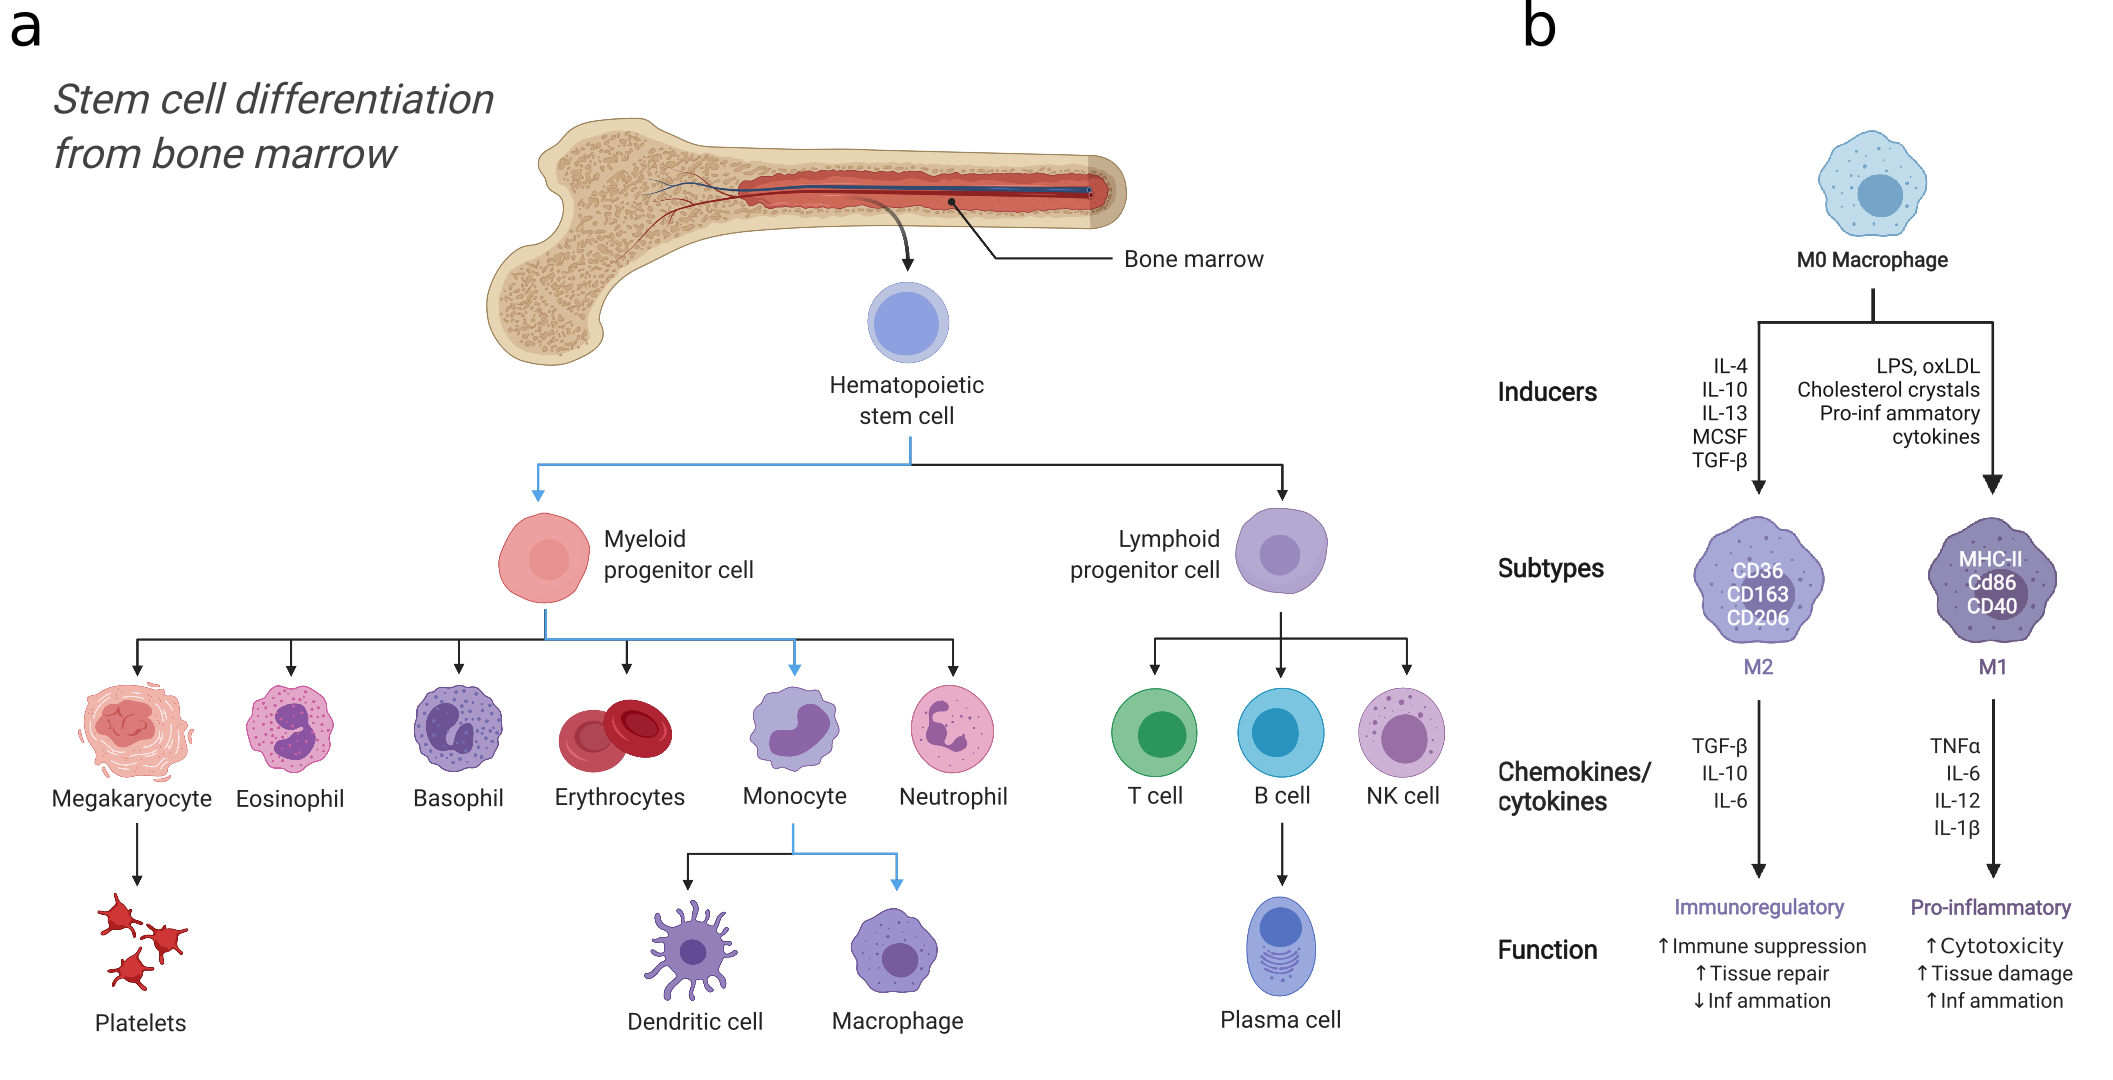
\includegraphics[width=\textwidth]{Parts/Part02/gfx/macrophage_differentiation.png}
    \caption[Macrophage differentiation.]{Macrophage differentiation from hematopoietic stem cells. \textbf{a:} Cellular differntiation pathway leading from bone marrow stem cells to macrophages \textbf{b:} Macrophage polarization from M0 to M1 (pro-inflammatory) or M2 (anti-inflammatory) macrophages. For either forms, molecules associated with induction of polarization, surface exposure and secretion are listed, as well as its functions.  Adapted from "Stem cell differentiation from bone marrow" and "Macrophage subtypes in atherosclerosis", by BioRender.com (2020). Retrieved from https://app.biorender.com/biorender-templates}
    \label{fig:02-03:macrophage}
\end{figure}


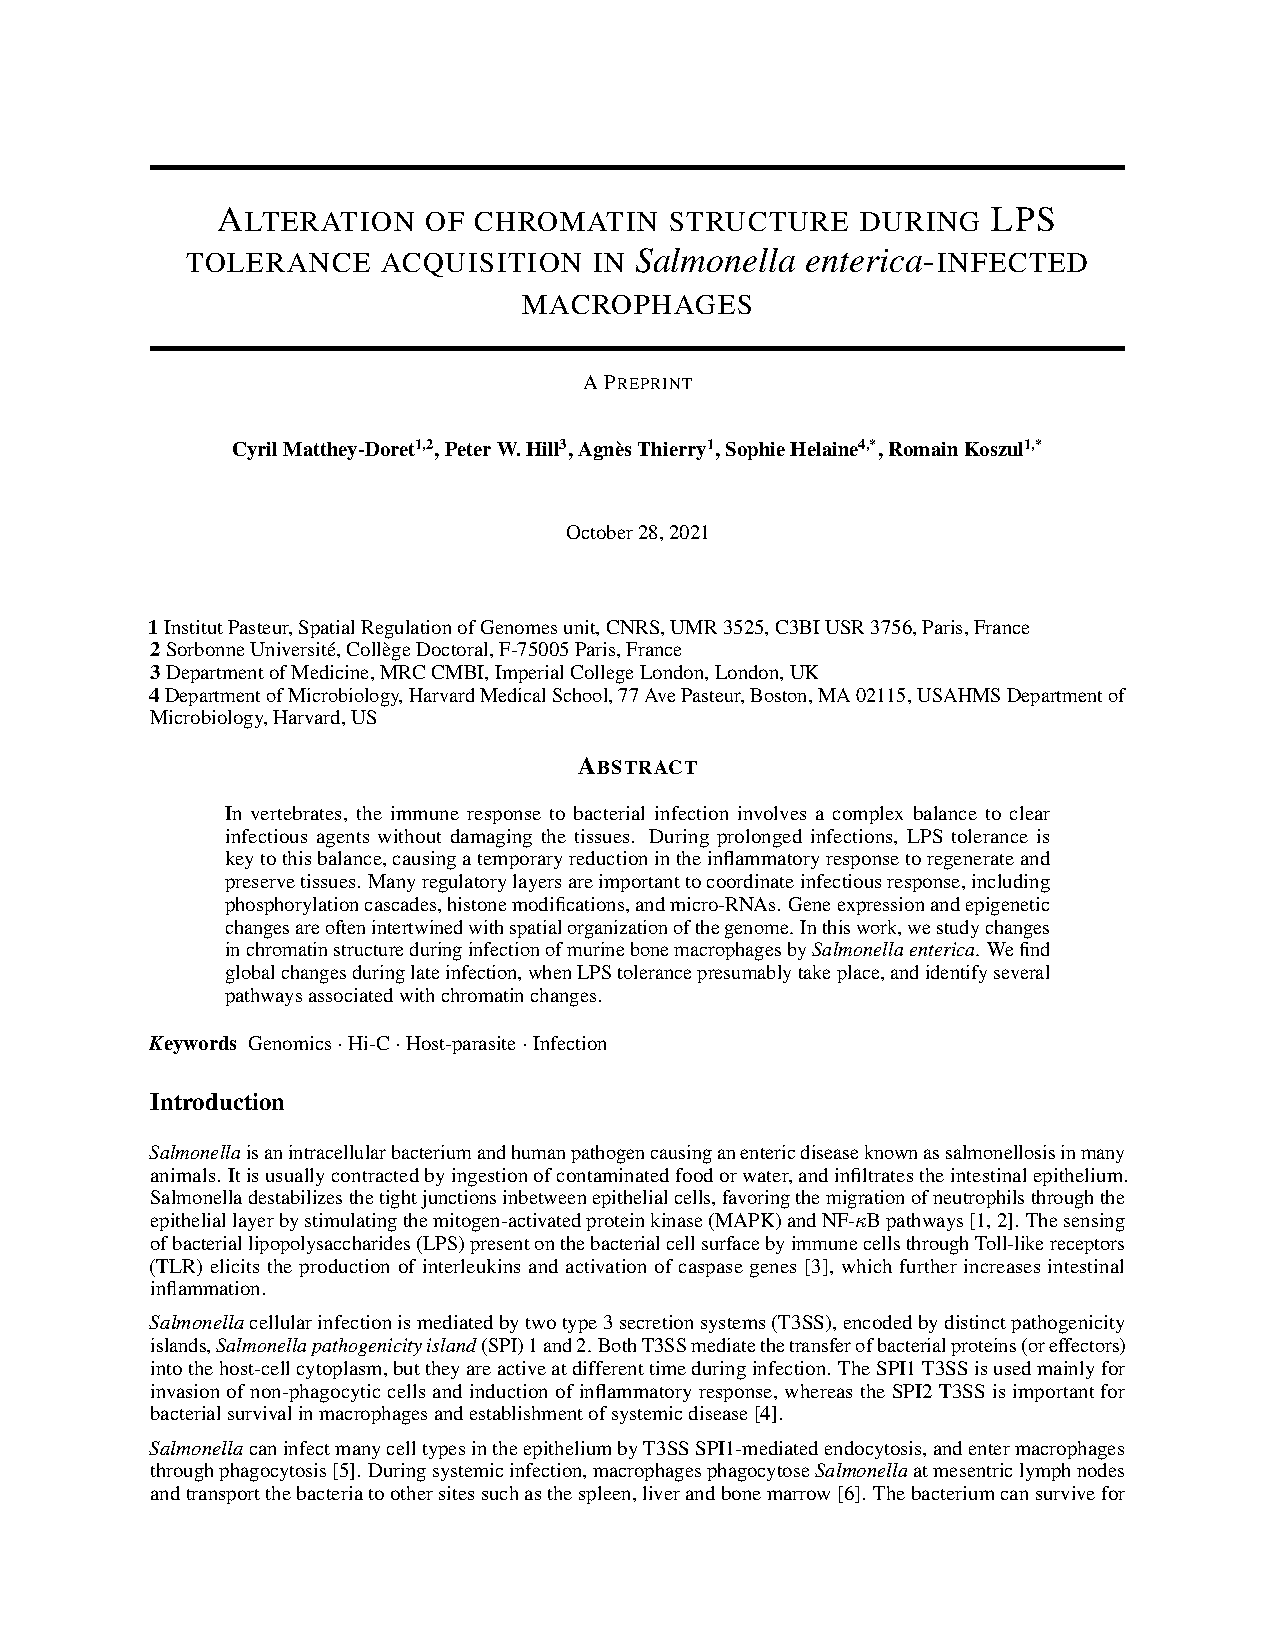
\includepdf[pages=-,addtotoc={
     1,section,1,Alteration of chromatin structure in macrophages during infection by \textit{Salmonella},p1,
     1,subsection,2,Introduction,p2,
     2,subsection,2,Results,p3,
     4,subsection,2,Discussion,p4,
     4,subsection,2,Methods,p5}]
     {Publications/mouse_salmonella_manuscript.pdf}    